\documentclass{article}
\usepackage{tikz}
\usepackage{mathrsfs}
\begin{document}
 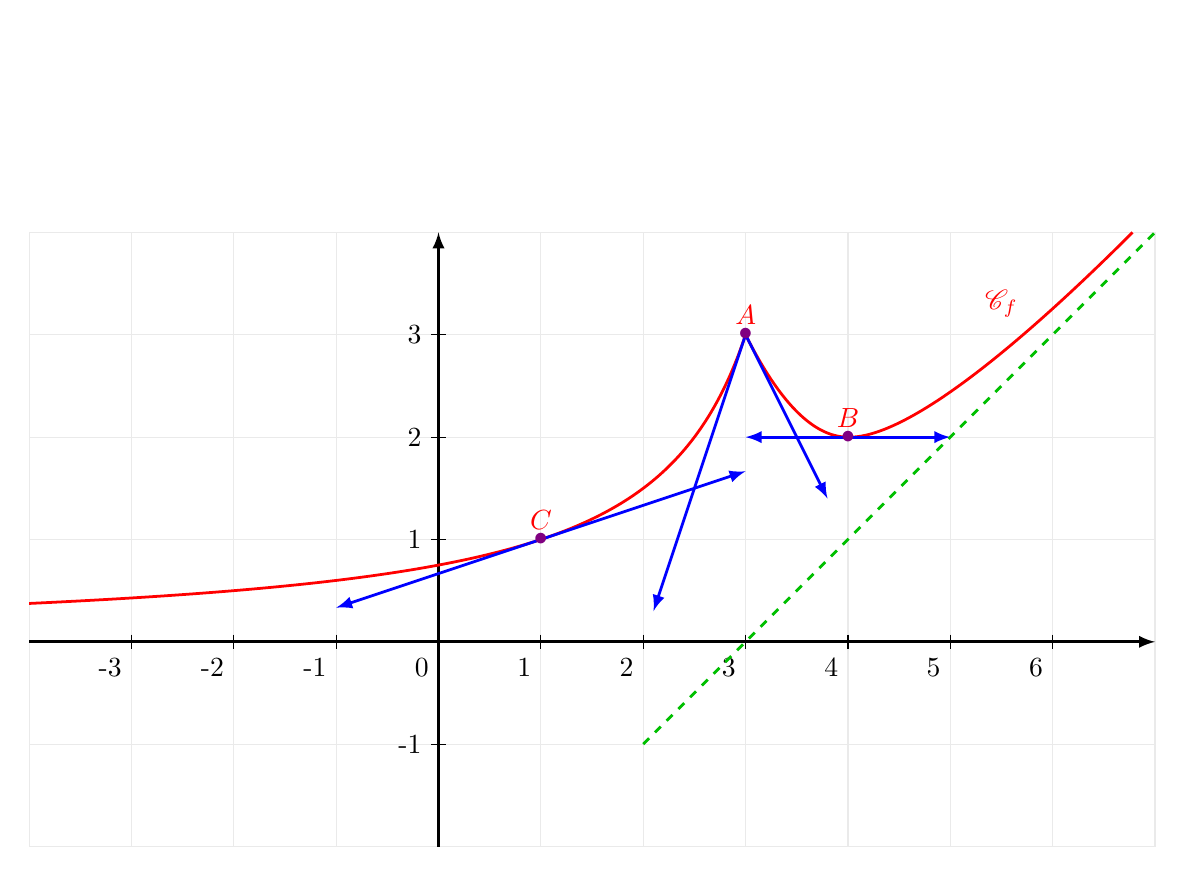
\begin{tikzpicture}[scale=1.3]
  \draw[opacity=0.3,gray!55] (-4,-2)grid(7,4);
  \draw[line width=1pt,-latex](-4,0)--(7,0);
  \draw[line width=1pt,-latex](0,-2)--(0,4);
  \foreach \i in{-3,...,6}
  \draw[shift={(\i,0)}](0,2pt)--(0,-2pt)node[below left]{\i};
  \foreach \j in{-1,1,2,3}
  \draw[shift={(0,\j)}](2pt,0)--(-2pt,0)node[left]{\j};
  \clip (-4,-2)rectangle(7,6);
   \draw[line width=1pt,red,smooth,samples=100,domain=-4:3]plot(\x,{-3/(\x-4)});
    \draw[line width=1pt,red,smooth,samples=100,domain=3:4]plot(\x,{(\x-4)*(\x-4)+2});   
%     \draw[line width=1pt,violet,smooth,samples=100,domain=4:7]plot(\x,{0.5*(\x-4)*(\x-4)+2});
     \draw[line width=1pt,red] (4,2).. controls (4.66,1.98) and (5.98,3.2)
 ..(6.78,4);
   \draw[blue,line width=1pt,latex-latex](-1,1/3)--(3,5/3);
    \draw[blue,line width=1pt,latex-](2.1,0.3)--(3,3);   
    \draw[blue,line width=1pt,latex-](3.8,1.4)--(3,3);    
    \draw[blue,line width=1pt, latex-latex](3,2)--(5,2);    
    \draw[green!75!black,line width=1pt,dashed](2,-1)--(7,4);
    \coordinate[label= above :\color{red}$A$,label=center:\color{violet}$ \bullet $ ](A) at (3,3);
    \coordinate[label= above :\color{red}$B$,label=center:\color{violet}$ \bullet $ ](B) at (4,2);
    \coordinate[label= above :\color{red}$C$,label=center:\color{violet}$ \bullet $ ](C) at (1,1);
       \node at (5.5,3.3){\color{red}$\mathscr C_f$};
 \end{tikzpicture}
\end{document}
